\documentclass[tikz,border=4pt]{standalone}

\usepackage{amsmath}
\usepackage{amssymb}
\usepackage{xcolor}
\usetikzlibrary{arrows.meta,positioning,calc,fit,backgrounds,decorations.pathreplacing}

\providecommand{\ket}[1]{|#1\rangle}
\providecommand{\bra}[1]{\langle #1|}

\begin{document}

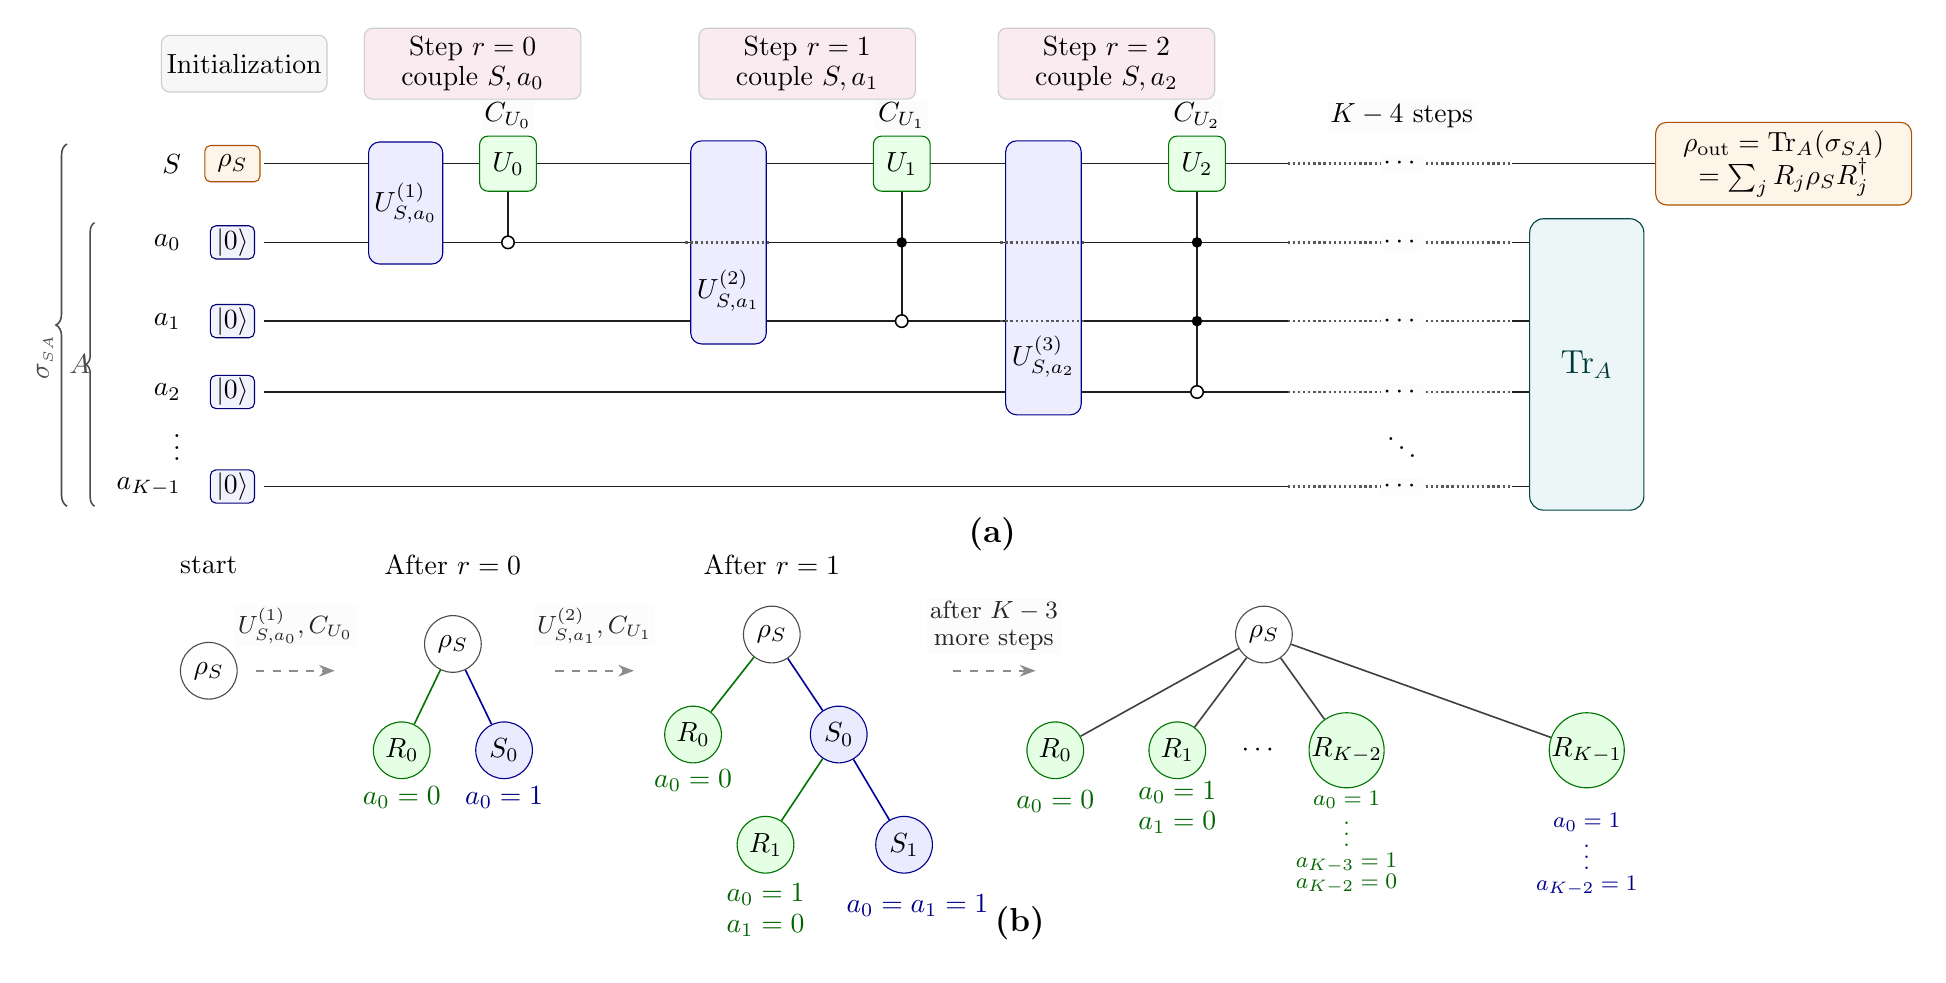
\begin{tikzpicture}[
    x=1cm,y=1cm,
    >=Stealth,
    font=\normalsize,
    wire/.style={line width=0.58pt, black!88},
    panel/.style={draw=black!32, rounded corners=5pt, line width=0.45pt, fill=black!1},
    header/.style={
        draw=black!20,
        rounded corners=3pt,
        fill=purple!8,
        minimum width=2.75cm,
        minimum height=0.90cm,
        align=center,
        font=\normalsize,
        inner sep=2pt
    },
    inithead/.style={
        draw=black!20,
        rounded corners=3pt,
        fill=black!3,
        minimum width=1.95cm,
        minimum height=0.72cm,
        align=center,
        font=\normalsize,
        inner sep=2pt
    },
    gateU/.style={
        draw=blue!55!black,
        rounded corners=4pt,
        fill=blue!7,
        minimum width=0.88cm,
        align=center,
        font=\normalsize,
        inner sep=2pt
    },
    gateUpiece/.style={
        draw=blue!55!black,
        rounded corners=3pt,
        fill=blue!7,
        minimum width=0.86cm,
        minimum height=0.50cm,
        align=center,
        inner sep=1pt
    },
    gateC/.style={
        draw=green!45!black,
        rounded corners=3pt,
        fill=green!9,
        minimum width=0.72cm,
        minimum height=0.70cm,
        align=center,
        font=\normalsize,
        inner sep=1.5pt
    },
    measbox/.style={
        draw=teal!55!black,
        rounded corners=5pt,
        fill=teal!7,
        minimum width=1.45cm,
        minimum height=3.70cm,
        align=center,
        inner sep=2pt
    },
    initbox/.style={
        draw=blue!45!black,
        rounded corners=2pt,
        fill=blue!5,
        minimum width=0.56cm,
        minimum height=0.40cm,
        inner sep=1pt
    },
    rhobox/.style={
        draw=orange!65!black,
        rounded corners=2pt,
        fill=orange!9,
        minimum width=0.70cm,
        minimum height=0.46cm,
        inner sep=1pt
    },
    outbox/.style={
        draw=orange!65!black,
        rounded corners=4pt,
        fill=orange!9,
        minimum width=3.25cm,
        minimum height=1.05cm,
        align=center,
        inner sep=2pt
    },
    dot/.style={circle, fill=black, inner sep=1.35pt},
    zerodot/.style={circle, draw=black, fill=white, line width=0.55pt, minimum size=4.5pt, inner sep=0pt},
    treeO/.style={
        circle,
        draw=black!70,
        fill=white,
        minimum size=7.2mm,
        inner sep=0pt
    },
    treeG/.style={
        circle,
        draw=green!45!black,
        fill=green!10,
        minimum size=7.2mm,
        inner sep=0pt
    },
    treeB/.style={
        circle,
        draw=blue!55!black,
        fill=blue!8,
        minimum size=7.2mm,
        inner sep=0pt
    },
    branchlab/.style={font=\normalsize, inner sep=1pt, fill=black!1},
    stateG/.style={font=\normalsize, align=center, text=green!40!black, inner sep=1pt},
    stateB/.style={font=\normalsize, align=center, text=blue!55!black, inner sep=1pt},
    applab/.style={font=\normalsize, align=center, text=black, inner sep=1pt},
    steplab/.style={font=\small, align=center, text=black!85, fill=black!1, inner sep=1pt},
    treeline/.style={line width=0.58pt, black!75},
    note/.style={
        draw=black!20,
        rounded corners=2pt,
        fill=black!2,
        align=center,
        inner sep=2pt
    },
    flowdash/.style={-{Stealth[length=2.0mm]}, line width=0.55pt, dashed, black!45}
]

% ============================================================
% Global dimensions
% ============================================================
\def\xL{0}
\def\xR{24.2}
\def\yTop{9.75}
\def\yMid{2.35}
\def\yBot{-3.75}

\path[fill=white] (-0.75,-2.10) rectangle (23.25,9.55);

% ============================================================
% Upper layer: compact circuit cartoon
% ============================================================

\def\yS{7.95}
\def\ya{6.95}
\def\yb{5.95}
\def\yc{5.05}
\def\yv{4.45}
\def\yk{3.85}

% Column headers
\node[inithead] at (2.00,9.22) {Initialization};
\node[header] at (4.90,9.22) {Step \(r=0\)\\[-1pt]couple \(S,a_0\)};
\node[header] at (9.15,9.22) {Step \(r=1\)\\[-1pt]couple \(S,a_1\)};
\node[header] at (12.95,9.22) {Step \(r=2\)\\[-1pt]couple \(S,a_2\)};

% Labels
\node[left] at (1.32,\yS) {$S$};
\node[left] at (1.32,\ya) {$a_0$};
\node[left] at (1.32,\yb) {$a_1$};
\node[left] at (1.32,\yc) {$a_2$};
\node[left] at (1.32,\yv) {$\vdots$};
\node[left] at (1.32,\yk) {$a_{K-1}$};
\draw[
    decorate,
    decoration={brace,amplitude=3.2pt},
    line width=0.55pt,
    black!70
] (0.1,\yk-0.25) -- (0.1,\ya+0.25)
node[midway,left=-2pt] {$A$};
\draw[
    decorate,
    decoration={brace,amplitude=4.0pt},
    line width=0.58pt,
    black!70
] (-0.25,\yk-0.25) -- (-0.25,\yS+0.25)
node[midway,left=8pt,rotate=90] {\(\sigma_{\scriptscriptstyle SA}\)};

% Inputs
\node[rhobox] at (1.85,\yS) {$\rho_S$};
\foreach \yy in {\ya,\yb,\yc,\yk}{
    \node[initbox] at (1.85,\yy) {$\ket{0}$};
}

% Wires
\draw[wire] (2.25,\yS) -- (20.65,\yS);
\foreach \yy in {\ya,\yb,\yc,\yk}{
    \draw[wire] (2.25,\yy) -- (16.80,\yy);
}

% ------------------------------------------------------------
% Step r=0: unitary on S,a0, then controlled feedback U0
% ------------------------------------------------------------
\node[gateU, minimum height=1.55cm] (U0split) at (4.05,{(\yS+\ya)/2})
{\(U^{(1)}_{S,a_0}\)};

\node[gateC] (U0fb) at (5.35,\yS) {$U_0$};
\draw[wire] (5.35,\ya) -- (U0fb.south);
\node[zerodot] at (5.35,\ya) {};
\node[font=\normalsize, inner sep=1pt, fill=black!1] at (5.35,8.56) {\(C_{U_0}\)};

% ------------------------------------------------------------
% Step r=1: controlled by a0, acts on S and a1, not on a0
% ------------------------------------------------------------
\node[gateU, minimum width=0.96cm, minimum height=2.58cm] (U1split)
    at (8.15,{(\yS+\yb)/2}) {};
\node[align=center, font=\normalsize] at (8.15,6.34)
    {\(U^{(2)}_{S,a_1}\)};
\draw[densely dotted, line width=0.85pt, black!65]
    (7.60,\ya) -- (8.70,\ya);

\node[gateC] (U1fb) at (10.35,\yS) {$U_1$};
\draw[wire] (10.35,\yb) -- (U1fb.south);
\node[dot] at (10.35,\ya) {};
\node[zerodot] at (10.35,\yb) {};
\node[font=\normalsize, inner sep=1pt, fill=black!1] at (10.35,8.56) {\(C_{U_1}\)};

% ------------------------------------------------------------
% Step r=2: controlled by a0,a1, acts on S and a2, not on a0,a1
% ------------------------------------------------------------
\node[gateU, minimum width=0.96cm, minimum height=3.48cm] (U2split)
    at (12.15,{(\yS+\yc)/2}) {};
\node[align=center, font=\normalsize] at (12.15,5.50)
    {\(U^{(3)}_{S,a_2}\)};
\draw[densely dotted, line width=0.85pt, black!65]
    (11.60,\ya) -- (12.70,\ya);
\draw[densely dotted, line width=0.85pt, black!65]
    (11.60,\yb) -- (12.70,\yb);

\node[gateC] (U2fb) at (14.10,\yS) {$U_2$};
\draw[wire] (14.10,\yc) -- (U2fb.south);
\node[dot] at (14.10,\ya) {};
\node[dot] at (14.10,\yb) {};
\node[zerodot] at (14.10,\yc) {};
\node[font=\normalsize, inner sep=1pt, fill=black!1] at (14.10,8.56) {\(C_{U_2}\)};

% ------------------------------------------------------------
% Dotted continuation for the omitted steps
% ------------------------------------------------------------
\foreach \yy in {\yS,\ya,\yb,\yc,\yk}{
    \draw[black!1, line width=1.6pt] (15.25,\yy) -- (18.10,\yy);
    \draw[densely dotted, line width=0.85pt, black!65] (15.25,\yy) -- (18.10,\yy);
    \node[fill=black!1, inner sep=1pt] at (16.70,\yy) {$\cdots$};
}
\node[font=\normalsize, fill=black!1, inner sep=1pt] at (16.70,8.56) {\(K-4\) steps};
\node at (16.70,\yv) {\(\ddots\)};

% ------------------------------------------------------------
% Measure ancillas, forget the result; system output remains
% ------------------------------------------------------------
\node[measbox] (Mbox) at (19.05,{(\ya+\yk)/2}) {};
\node[align=center, font=\large, text=teal!45!black] at (19.05,{(\ya+\yk)/2})
{\(\operatorname{Tr}_A\)};

\foreach \yy in {\ya,\yb,\yc,\yk}{
    \draw[wire] (18.10,\yy) -- (Mbox.west |- 0,\yy);
}
\draw[wire] (19.75,\yS) -- (19.95,\yS);
\node[outbox] at (21.55,\yS)
{\(\rho_{\rm out}=\operatorname{Tr}_A(\sigma_{SA})\)\\[-1pt]
\(\textstyle=\sum_j R_j\rho_S R_j^\dagger\)};

\node[font=\large\bfseries] at (11.50,3.25) {(a)};

% ============================================================
% Lower layer: branch/state interpretation
% ============================================================
\begin{scope}[yshift=1.35cm]

\node at (1.55,1.50) {start};
\node at (4.65,1.50) {After \(r=0\)};
\node at (8.70,1.50) {After \(r=1\)};

% Start
\node[treeO] (T0) at (1.55,0.16) {$\rho_S$};
\draw[flowdash] (2.15,0.16) -- (3.15,0.16);
\node[steplab] at (2.65,0.73) {\(U^{(1)}_{S,a_0}, C_{U_0}\)};

% After r=0
\node[treeO] (A0) at (4.65,0.50) {$\rho_S$};
\node[treeG] (A1) at (4.00,-0.85) {$R_0$};
\node[treeB] (A2) at (5.30,-0.85) {$S_0$};
\draw[treeline, green!45!black] (A0) -- (A1);
\draw[treeline, blue!60!black] (A0) -- (A2);
\node[stateG] at (4.00,-1.45) {\(a_0=0\)};
\node[stateB] at (5.30,-1.45) {\(a_0=1\)};
\draw[flowdash] (5.95,0.16) -- (6.95,0.16);
\node[steplab] at (6.45,0.73) {\(U^{(2)}_{S,a_1}, C_{U_1}\)};

% After r=1
\node[treeO] (B0) at (8.70,0.62) {$\rho_S$};
\node[treeG] (B1) at (7.70,-0.65) {$R_0$};
\node[treeB] (B2) at (9.55,-0.65) {$S_0$};
\node[treeG] (B3) at (8.62,-2.05) {$R_1$};
\node[treeB] (B4) at (10.38,-2.05) {$S_1$};
\draw[treeline, green!45!black] (B0) -- (B1);
\draw[treeline, blue!60!black] (B0) -- (B2);
\draw[treeline, green!45!black] (B2) -- (B3);
\draw[treeline, blue!60!black] (B2) -- (B4);
\node[stateG] at (7.70,-1.23) {\(a_0=0\)};
\node[stateG] at (8.62,-2.88) {\(a_0=1\)\\[-1pt]\(a_1=0\)};
\node[stateB] at (10.55,-2.82) {\(a_0=a_1=1\)};
\draw[flowdash] (11.00,0.16) -- (12.05,0.16);
\node[steplab] at (11.52,0.73) {after \(K-3\)\\[-1pt]more steps};

% After omitted steps
\node[treeO] (C0) at (14.95,0.62) {$\rho_S$};
\node[treeG] (C1) at (12.30,-0.85) {$R_0$};
\node[treeG] (C2) at (13.85,-0.85) {$R_1$};
\node at (14.90,-0.85) {$\cdots$};
\node[treeG] (C3) at (16.00,-0.85) {$R_{K-2}$};
\node[treeG] (C4) at (19.05,-0.85) {$R_{K-1}$};
\draw[treeline] (C0) -- (C1);
\draw[treeline] (C0) -- (C2);
\draw[treeline] (C0) -- (C3);
\draw[treeline] (C0) -- (C4);
\node[stateG] at (12.30,-1.50) {\(a_0=0\)};
\node[stateG] at (13.85,-1.58) {\(a_0=1\)\\[-1pt]\(a_1=0\)};
\node[stateG, font=\footnotesize] at (16.00,-2.02) {\(a_0=1\)\\[-2pt]\(\vdots\)\\[-2pt]\(a_{K-3}=1\)\\[-2pt]\(a_{K-2}=0\)};
\node[stateB, font=\footnotesize] at (19.05,-2.18) {\(a_0=1\)\\[-2pt]\(\vdots\)\\[-2pt]\(a_{K-2}=1\)};

\node[font=\large\bfseries] at (11.85,-3.05) {(b)};

\end{scope}

\end{tikzpicture}

\end{document}
